\chapter{Finite element assembly}
\label{sec:assembly}

\newtheorem{example}{\small{\sc{Example}}}[section]

In this section, we present a general algorithm for assembly of finite
element variational forms and define the concepts which the UFC
interface is based on.

\section{An introductory example}
\index{Poisson's equation}
\index{variational problem}

As an introduction, consider Poisson's equation,
\begin{equation}
  \label{eq:poisson}
  \begin{split}
  - \Delta u &= f, \quad \mbox{ in } \Omega, \\
  u &= 0, \quad \mbox{ on } \partial\Omega.
  \end{split}
\end{equation}
For $v \in \hat{V}$ a test function, we multiply (\ref{eq:poisson}) by
$v$ and integrate by parts to obtain the variational problem: Find $u
\in V$ such that
\begin{equation} \label{eq:poissonvariational}
  \int_{\Omega} \nabla v \cdot \nabla u \dx = \int_{\Omega} v f \dx
  \quad \forall v \in \hat{V},
\end{equation}
which we may restate as: Find $u \in V$ such that
\begin{equation}
  a(v, u) = L(v) \quad \forall v \in \hat{V},
\end{equation}
where the \emph{bilinear form} $a : \hat{V} \times V \rightarrow \R$
is given by
\begin{equation}
  a(v, u) = \int_{\Omega} \nabla v \cdot \nabla u \dx,
\end{equation}
and the \emph{linear form} $L : \hat{V} \rightarrow \R$ is given by
\begin{equation}
  L(v) = \int_{\Omega} v f \dx.
\end{equation}

\index{test space}
\index{trial space}
By replacing the test space $\hat{V}$ and the trial space $V$ with a
pair of discrete test and trial spaces $\hat{V}_h$ and $V_h$, we
obtain the discrete variational problem: Find $U \in V_h$ such that
\begin{equation}
  a(v, U) = L(v) \quad \forall v \in \hat{V}_h.
\end{equation}
To obtain the discrete solution $U \in V_h$, we make an Ansatz
 for $U$ as a linear combination of a
suitable set of basis functions $\{\phi_j\}_{j=1}^N$ for $V_h$,
\begin{equation}
  U(x) = \sum_{j=1}^N U_j \phi_j(x),
\end{equation}
and take $v = \phi_i$ for $i = 1,2,\ldots,N$ for
$\{\hat{\phi}_i\}_{i=1}^N$ a set of basis functions for the test space
$V_h$. We thus obtain the linear system
\begin{equation}
  a(\hat{\phi}_i, \sum_{j=1}^N U_j \phi_j) = L(\hat{\phi}_i), \quad i = 1,2,\ldots,N,
\end{equation}
or, since $a$ is bilinear,
\begin{equation}
  A U = b,
\end{equation}
where
\begin{eqnarray}
  A_{ij} &=& a(\hat{\phi}_i, \phi_j), \quad i = 1,2,\ldots,N, j = 1,2,\ldots,N, \\
  b_i &=& L(\hat{\phi}_i), \quad i = 1,2,\ldots,N.
\end{eqnarray}

\section{Discretization of variational forms}

\subsection{The Finite Element}
\index{finite element}

A finite element is mathematically defined as a triplet consisting
of a polygon, a function space, and a set of linear functionals. 
Given that the dimension of the function space and the number of
the (linearly independent) linear functionals are equal, the
finite element is uniquely defined. 
With this definition of a finite element, the basis functions
are implicitly defined as the solution of a linear system.

We take our starting point in the standard Ciarlet
definition~\cite{Cia78}, but consider a finite element with a fixet
set of basis functions.  These basis functions are pre-computed from
the triplet mentioned above. Hence, we will refer to a finite
element as a collection of
\begin{itemize}
\item a polygon,  
\item a set of basis functions $\{\phi_i\}_{i=1}^n$ and
the derivatives of those basis functions,
\item the degrees of freedom, which are linear functionals, $L_i : V
\rightarrow \R, i = 1, 2, \ldots, n$, where $V = \mathrm{span}\{\phi_i\}_{i=1}^n$.  Usually,
$L_i$ may be extended from $V$ to an appropriate Sobolev space.
\end{itemize}
In addition, our finite element will contain functionality
for interpolation. 

\subsection{Variational forms}
\index{variational form}

In general, we shall be concerned with the discretization of general
variational forms of arity~$r > 0$,
\begin{equation} \label{eq:variationalform}
  a : V_h^1 \times V_h^2 \times \cdots \times V_h^r \times
  W_h^1 \times W_h^2 \times \cdots \times W_h^n \rightarrow \R.
\end{equation}
defined on the product space $V_h^1 \times V_h^2 \times \cdots \times
V_h^r \times W_h^1 \times W_h^2 \times \cdots \times W_h^n$ of two sets
$\{V_h^j\}_{j=1}^r, \{W_h^j\}_{j=1}^n$ of discrete function spaces on
a triangulation $\mathcal{T}$ of a domain $\Omega \subset \R^d$. 
We also often write this as 
\begin{equation}
a = a(v_1, \ldots, v_r; w_1, \ldots, w_n), 
\end{equation}
where ';' is used to separate the $V_h$ spaces from the $W_h$ spaces. 
The distinction between the spaces $\{V_h^j\}_{j=1}^r$ and
$\{W_h^j\}_{j=1}^n$ lies in how the discretization is made for each
set of spaces. This will be explained below.

In the simplest case, all function spaces are equal but there are many
important examples, such as mixed methods, where it is important to
consider arguments coming from different function spaces.

Let $\mathcal{T} = \{K\}$ be a set of disjoint \emph{cells} (a
triangulation) partitioning a domain $\cup_{K\in\mathcal{T}} K =
\Omega \subset \R^d$, let $\partial_e \mathcal{T}$ denote the set of
\emph{exterior facets} (the set of cell facets
incident with the boundary $\partial \Omega$), and let $\partial_i
\mathcal{T}$ denote the set of $\emph{interior facets}$ (the set of
cell facets non-incident with the boundary $\partial \Omega$).

We shall assume that the variational form~(\ref{eq:variationalform})
may be expressed as a sum of integrals over the cells~$\mathcal{T}$,
the exterior facets~$\partial_i \mathcal{T}$ and the interior
facets~$\partial_e \mathcal{T}$. We shall allow integrals expressed on
disjoint subsets $\{\mathcal{T}_k\}_{k=1}^{n_c}$, $\{\partial_e
\mathcal{T})_k\}_{k=1}^{n_e}$ and $\{\partial_i
\mathcal{T}_k\}_{k=1}^{n_i}$ of $\mathcal{T}$, $\partial_e
\mathcal{T}$ and $\partial_i \mathcal{T}$ respectively.

We thus assume that the form $a$ is given by
\begin{equation}
  \begin{split}
    a(v_1, \ldots, v_r; w_1, \ldots,  w_n)
    &=
    \sum_{k=1}^{n_c} \sum_{K\in\mathcal{T}_k} \int_{K}
    I^c_k(v_1, \ldots, v_r; w_1, \ldots w_n) \dx \\
    &+
    \sum_{k=1}^{n_e} \sum_{S\in\partial_e\mathcal{T}_k} \int_{S}
    I^e_k(v_1, \ldots, v_r; w_1, \ldots,  w_n) \ds \\
    &+
    \sum_{k=1}^{n_i} \sum_{S\in\partial_i\mathcal{T}_k} \int_{S}
    I^i_k(v_1, \ldots, v_r; w_1, \ldots, w_n) \ds.
  \end{split} \label{eq:form_integrals}
\end{equation}
We refer to an integral over a cell~$K$ as a \emph{cell integral},
an integral over an exterior facet~$S$ as an \emph{exterior facet integral},
and to an integral over an interior facet~$S$ as an \emph{interior facet integral}.

\subsection{Discretization}
\label{sec:Discretization}
\index{discretization}

To discretetize the form $a$, we let
$\{\phi_i^1\}_{i=1}^{N^1},
 \{\phi_i^2\}_{i=1}^{N^2}, \ldots,
 \{\phi_i^r\}_{i=1}^{N^r}$
be bases of $V_h^1, V_h^2, \ldots, V_h^r$ respectively and let $i =
(i_1, i_2, \ldots, i_r)$ be a multiindex of length $|i| = r$. The
form $a$ then defines a rank~$r$ tensor given by
\begin{equation} \label{eq:tensor}
  A_i = a(\phi_{i_1}^1, \phi_{i_2}^2, \ldots, \phi_{i_r}^r; w_1, w_2, \ldots, w_n)
  \quad \forall i \in \mathcal{I},
\end{equation}
where $\mathcal{I}$ is the index set
\begin{equation}
  \mathcal{I} = 
  \prod_{j=1}^r[1,|V^j_h|] = \{(1,1,\ldots,1), (1,1,\ldots,2), \ldots,
  (N^1,N^2,\ldots,N^r)\}.
\end{equation}
For any given form of arity~$r$, the tensor~$A$ is a
(typically sparse) tensor of rank~$r$ and dimension
$|V_h^1| \times |V_h^2| \times \ldots \times |V_h^r|
= N^1 \times N^2 \times \ldots \times N^r$.
\index{global tensor}

Typically, the arity of the form~$a$ is $r = 0$, $r = 1$
or $r = 2$. When $r = 0$, the corresponding (rank zero) tensor is a
scalar, when $r = 1$, the corresponding (rank one) tensor is a vector
(the ``load vector'') and when $r = 2$, the corresponding (rank two)
tensor is a matrix (the ``stiffness matrix'').
Forms of higher arity also appear, though they are rarely assembled as
a higher-dimensional sparse tensor.

Note here that we consider the functions $w_1, w_2, \ldots, w_n$ as
fixed in the sense that the discrete operator is computed for a given
set of functions, which we refer to as \emph{coefficients}. As an
example, consider again the variational
problem~(\ref{eq:poissonvariational}) for Poisson's equation. For the
bilinear form~$a$, the arity (rank) is $r = 2$ and the number of
coefficients is $n = 0$, while for the linear form~$L$, the arity is
$r = 1$ and the number of coefficients is $n = 1$. We may also choose
to directly compute the action of the bilinear form $a$ obtained by
assembling a vector from the form
\begin{equation}
  a(v_1; w_1) = \int_{\Omega} v_1 w_1 \dx,
\end{equation}
where now $r = 1$ and $n = 1$.

We list below a few other examples to illustrate the notation.

\begin{example}
\label{example:div}
Our first example is related
to the divergence constraint in fluid flow. Let $a$ be given by
\begin{equation}
a(q, u) = \int_{\Omega} q \nabla \cdot u \dx, \quad q\in V_h^1, \quad u\in V_h^2, 
\end{equation}
where $V_h^1$ is a space of scalar-valued functions and
where $V_h^2$ is a space of vector-valued functions.
The form $a : V_h^1 \times V_h^2  \rightarrow \R$ is bilinear and
thus $r = 2$. Furthermore, the form does not depend on any
coefficients and thus $n=0$.   
\end{example}

\begin{example}
\label{example:nonlinearconv}
Another common form in fluid flow (with variable density) is: 
\begin{equation}
a(v,u;w,\varrho) = \int_{\Omega} v \, \varrho \, w \cdot \nabla  u \dx. 
\end{equation}
Here, $v\in V_h^1,\ u \in V_h^2,\ w\in W_h^1, \ \varrho \in W_h^2$, where
$V_h^1$, $V_h^2$, and $W_h^1$ are spaces of vector-valued functions, while $W_h^2$ is a space of  
scalar-valued functions. 
The form takes four arguments, where two of the arguments
are coefficients,
\begin{equation}
a : V_h^1 \times V_h^2 \times W_h^1 \times W_h^2 \rightarrow \R.
\end{equation}
Hence, $r=2$ and $n=2$. 
\end{example}

\begin{example}
\label{example:rhs}
The form corresponding to the right-hand side of Poisson's equation
(and other scalar equations) is given by
\begin{equation}
a(v; f) = \int_{\Omega} v f \dx.
\end{equation}
The form takes two arguments and one of them is a coefficient,
\begin{equation}
a : V_h^1 \times  W_h^1 \rightarrow \R.
\end{equation}
Hence, $r = n = 1$.
\end{example}

\begin{example}
The $H^1$ norm of the error $e = U - u$ squared is: 
\begin{equation}
a(U, u) = \int_{\Omega} (U - u)^2 + |\nabla (U - u)|^2 \dx.
\end{equation}
The form takes two argumentsa and both are coefficients,,
\begin{equation}
a : W_h^1 \times  W_h^2 \rightarrow \R.
\end{equation}
Thus, $r=0$ and $n=2$. 
\end{example}

\section{Assembling the discrete operator}
\index{assembly}

The standard algorithm~\cite{ZieTay67,Hug87,Lan99} for computing
the global tensor~$A$ is known as \emph{assembly}; it is
computed by iterating over the cells $\mathcal{T}$, 
the exterior facets $\partial_e\mathcal{T}$ and
interior facets $\partial_i\mathcal{T}$, and adding from each
the local contribution to the global sparse tensor $A$.

For simplicity, consider the assembly of the global sparse tensor~$A$
corresponding to a form~$a$ given by a single integral
over all cells $\mathcal{T}$,
\begin{equation}
  a(v_1, v_2, \ldots, v_r; w_1, w_2, \ldots, w_n) =
  \sum_{K\in\mathcal{T}} \int_K
  I^c(v_1, v_2, \ldots, v_r; w_1, w_2, \ldots, w_n) \dx.
\end{equation}
The global sparse tensor~$A$ is then given by
\begin{equation}
  A_i = \sum_{K\in\mathcal{T}} \int_K
  I^c(\phi^1_{i_1}, \phi^2_{i_2}, \ldots, \phi^r_{i_r}; w_1, w_2, \ldots, w_n) \dx.
\end{equation}

To see how to compute the tensor $A$ by summing the local
contributions from each cell~$K$, we let $n^j_K = |\mathcal{P}_K|$
denote the dimension of the local finite
element space on $K$. Furthermore, let
\begin{equation}
  \iota_K^j : [1,n_K^j] \rightarrow [1,N^j] \label{eq:iota_K}
\end{equation}
denote the local-to-global mapping for each discrete
function space $V_h^j$, $j=1,2,\ldots,r$, and define for each $K \in
\mathcal{T}$ the collective local-to-global mapping $\iota_K :
\mathcal{I}_K \rightarrow \mathcal{I}$ by
\begin{equation}
  \iota_K(i) =
  (\iota_K^1(i_1),\iota_K^2(i_2),\ldots,\iota_K^r(i_r))
  \quad \forall i \in \mathcal{I}_K,
\end{equation}
where $\mathcal{I}_K$ is the index set
\begin{equation}
  \mathcal{I}_K = 
  \prod_{j=1}^r[1,|\mathcal{P}_K^j|] = \{(1,1,\ldots,1), (1,1,\ldots,2), \ldots,
  (n_K^1,n_K^2,\ldots,n_K^r)\}.
\end{equation}
Furthermore, for each $V_h^j$ we let $\{\phi^{K,j}_i\}_{i=1}^{n_K^j}$
denote the restriction to an element $K$ of the subset of the basis
$\{\phi_i^j\}_{i=1}^{N^j}$ of $V_h^j$ supported on $K$.

We may now compute~$A$ by summing the contributions from
each local cell~$K$,
\begin{equation}
  \begin{split}
  A_{\iota_K(i)}
  &=
  \sum_{K\in\mathcal{T}} \int_K
  I^c(\phi_{\iota_K(i_1)}^1, \phi_{\iota_K(i_2)}^2, \ldots, \phi_{\iota_K(i_r)}^r) \dx \\
  &=
  \sum_{K\in\mathcal{T}} \int_K
  I^c(\phi_{i_1}^{K,1},
      \phi_{i_2}^{K,2}, \ldots,
      \phi_{i_r}^{K,r}) \dx
  =
  \sum_{K\in\mathcal{T}}
  A^K_i,
  \end{split}
\end{equation}
where $A^K$ is the local \emph{cell tensor} on cell $K$ (the ``element
stiffness matrix''). Similarly, we may sum the local contributions
from the exterior and interior facets in the form of local
\emph{exterior facet tensors} and \emph{interior facet tensors}.
\index{cell tensor}
\index{exterior facet tensor}
\index{interior facet tensor}

\begin{figure}[htbp]
  \begin{center}
    \psfrag{i0}{\hspace{-0.5cm}$\iota_K^1(1)$}
    \psfrag{i1}{\hspace{-0.5cm}$\iota_K^1(2)$}
    \psfrag{i2}{\hspace{-0.5cm}$\iota_K^1(3)$}
    \psfrag{j0}{\hspace{-0.3cm}$\iota_K^2(1)$}
    \psfrag{j1}{\hspace{-0.5cm}$\iota_K^2(2)$}
    \psfrag{j2}{\hspace{-0.1cm}$\iota_K^2(3)$}
    \psfrag{A21}{$A^K_{32}$}
    \psfrag{1}{$1$}
    \psfrag{2}{$2$}
    \psfrag{3}{$3$}
    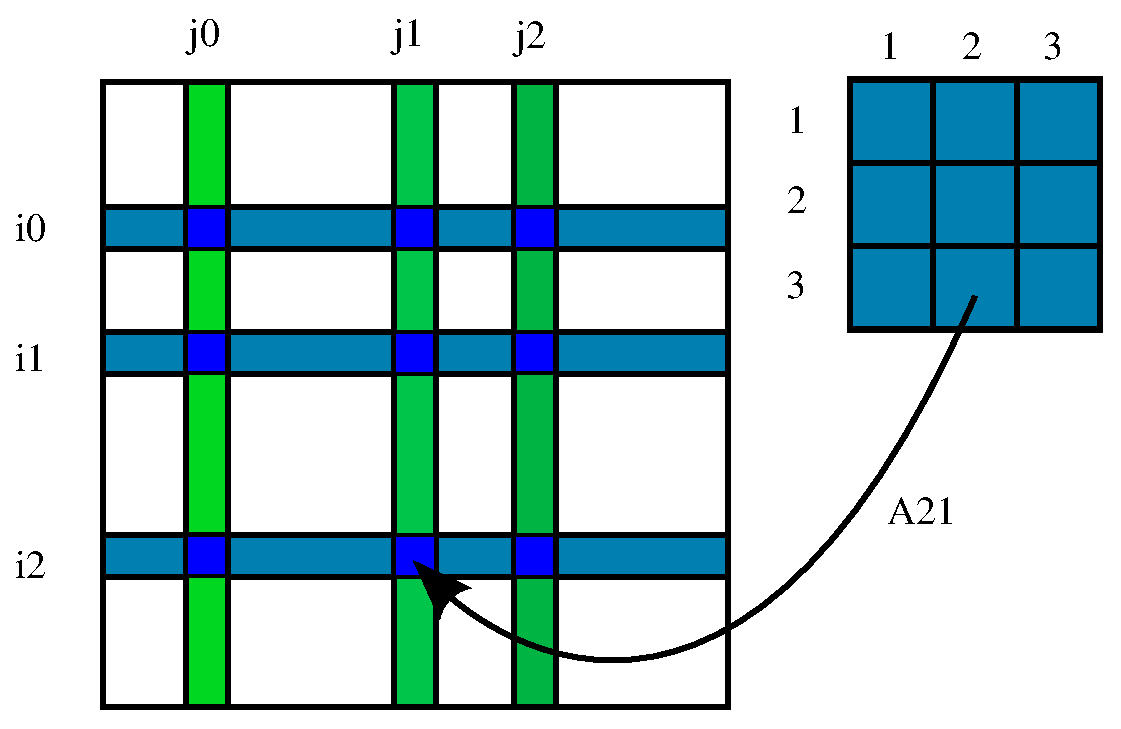
\includegraphics[height=3in]{eps/insertion.eps}
    \caption{Adding the entries of a cell tensor~$A^K$ to the
      global tensor~$A$ using the  local-to-global mapping
      $\iota_K$, illustrated here for a rank two
      tensor (a matrix).}
    \label{fig:insertion}
  \end{center}
\end{figure}

In Algorithm~\ref{alg:assembly}, we present a general algorithm for
assembling the contributions from the local cell, exterior facet and
interior facet tensors into a global sparse tensor. In
Appendix~\ref{app:assembly}, we present a sketch of the corresponding
implementation in C++ based on UFC. In both cases, we iterate over the
local cells, exterior and interior facets. On each local entity, we
compute the local tensor and add it to the global tensor as in
Figure~\ref{fig:insertion}.

\begin{algorithm}
$A = 0$ \\
\\
\emph{Assemble contributions from all cells} \\
\textbf{for each} $K \in \mathcal{T}$ \\
\\
\tab \textbf{for} $j = 1,2,\ldots,r$: \\
\tab\tab Tabulate the local-to-global mapping $\iota_K^j$ \\
\\
\tab Let $K \in \mathcal{T}_k$ \\
\tab Tabulate the cell tensor $A^K$ for $I^c_k$ \\
\tab Add $A^K_i$ to $A_{\iota_K^1(i_1), \iota_K^2(i_2), \ldots, \iota_K^r(i_r)}$ for all $i\in I_K$ \\
\\
\emph{Assemble contributions from all exterior facets} \\
\textbf{for each} $S \in \partial_e\mathcal{T}$ \\
\\
\tab \textbf{for} $j = 1,2,\ldots,r$: \\
\tab\tab Tabulate the local-to-global mapping $\iota_K^j$ \\
\\
\tab Let $S \in \partial_e\mathcal{T}_k$ \\
\tab Tabulate the exterior facet tensor $A^S$ for $I^e_k$ \\
\tab Add $A^S_i$ to $A_{\iota_K^1(i_1), \iota_K^2(i_2), \ldots, \iota_K^r(i_r)}$ for all $i\in I_K$ \\
\\
\\
\emph{Assemble contributions from all interior facets} \\
\textbf{for each} $S \in \partial_i\mathcal{T}$ \\
\\
\tab \textbf{for} $j = 1,2,\ldots,r$: \\
\tab\tab Tabulate the local-to-global mapping $\iota_K^j$ \\
\\
\tab Let $S \in \partial_i\mathcal{T}_k$ \\
\tab Tabulate the interior facet tensor $A^S$ for $I^i_k$ \\
\tab Add $A^S_i$ to $A_{\iota_K^1(i_1), \iota_K^2(i_2), \ldots, \iota_K^r(i_r)}$ for all $i\in I_K$ \\
\caption{Assembling the global tensor~$A$ from the local contributions
  on all cells, exterior and interior facets. For assembly over
  exterior facets, $K$ refers to the cell $K\in\mathcal{T}$ incident
  to the exterior facet~$S$, and for assembly over interior facets,
  $K$ refers to the ``macro cell'' consisting of the pair of cells
  $K^+$ and $K^-$ incident to the interior facet~$S$.}
\label{alg:assembly}
\end{algorithm}
